%\documentclass[onecolumn]{IEEEtranTIE}
\documentclass[journal]{IEEEtranTIE}
\usepackage{graphicx}
\usepackage{cite}
\usepackage{picinpar}
\usepackage{amsmath}
\usepackage{url}
\usepackage{flushend}
\usepackage[latin1]{inputenc}
\usepackage{colortbl}
\usepackage{soul}
\usepackage{multirow}
\usepackage{pifont}
\usepackage{color}
\usepackage{alltt}
\usepackage[hidelinks]{hyperref}
\usepackage{enumerate}
\usepackage{siunitx}
\usepackage{breakurl}
\usepackage{epstopdf}
\usepackage{pbox}

\begin{document}
\title{	ConAuth - context for authentication \\ (Dec. 2017)}

\author{
	\vskip 1em
	{
	Saurabh Sharma, \emph{saurabh.sharma@sv.cmu.edu}\\
	Omar Serrano, \emph{omar.serrano@sv.cmu.edu}
	}
}

\maketitle

\begin{abstract}
With the growing number of wireless devices, we need efficient mechanisms to let
the wireless devices communicate securely. The wireless devices sometimes share
common sensors that can be leveraged to perform additional authentication
procedures on a set of localized wireless devices. The problem which prevents
such a judicious use of sensors is the orientation of wireless devices. Sensors
such as gyroscope and accelerometer are commonly found in wireless devices, but
their readings make no sense until their orientations are the same. We plan to
conduct controlled experiments to investigate how different environmental factors
impact the accelerometer performance and how the best accuracy can be achieved
in an appropriate condition range. We also characterize the nature of an
accelerometer to understand its performance in different conditions. Based on
such comprehensive understanding, we propose to estimate the phone attitude and
provide for opportunistic calibration of the accelerometer
\end{abstract}

\begin{IEEEkeywords}
Contextual security, sensor funsion, Madgwick, device orientation.
\end{IEEEkeywords}

\definecolor{limegreen}{rgb}{0.2, 0.8, 0.2}
\definecolor{forestgreen}{rgb}{0.13, 0.55, 0.13}
\definecolor{greenhtml}{rgb}{0.0, 0.5, 0.0}

\section{Introduction}

\IEEEPARstart{W}{ith}
the growing number of IoT devices, securely pairing a new device into an
existing set of devices is an extremely important yet burdensome task.
Traditionally, these devices are paired manually, where an operator sets up an
authentication with the existing network of devices. Specifically, we address
the problem of a platoon ghost attack wherein an attacker device spoofs presence
within a platoon to gain admission and subsequently execute malicious attacks
\cite{Han}. To address such concerns, we explore the notion of fingerprinting
device sensor readings for a device's context.

Devices that share context are expected to experience similar events. For
example, two magnetometers in proximity are likely to processes similar events
if a magnetic strip is drawn close to them. Even if the readings are not exactly
the same, the devices are likely to exhibit similar patterns as a result of the
magnetic disturbance caused by the magnetic strip. Two video cameras, despite
having different points of view, might be able to determine that they share
context on the basis that both of them detect an object with similar shape and
color; for example, if one of the video cameras records an invidual with a blue
shirt walking toward it, and the other camera records an invidual with a blue
shirt walking away from it.

There is a wide range of possibilities in how devices and sensors are used to
determine context from a wide variety of physical stimuli, or how the scale of
context is defined (e.g., school building vs a single room); however, we limit
our research to the small context of a car, and to 3-dimensional orientation,
acceleration, and magnetic sensor readings. Instead of relying on traditional
methods (e.g, Kalam filter) to determine context from the type of sensors we are
using, we employ a convolutional neural network, a popular technique for solving
computer vison problems, to create a predictive model.

\section{Problem Statement}

With near-ubiquitous availability of wireless devices equipped with a wide
variety of sensors, research in building context aware services has been
growing. However, despite a large number of services proposed and developed as
research prototypes, the number of truly context-aware applications available in
wireless devices is quite limited. A major barrier for the large-scale
proliferation of context aware applications is poor accuracy \cite{Alanezi}.
We address one of the key reasons for this poor accuracy, which is the impact of
sensor orientation.

Devices have their sensors oriented in different positions. We first show that
smartphone positions significantly affect the values of the
sensor data being collected by a context aware application, and this in turn
has a significant impact on the accuracy of the application \cite{Alanezi}.
Next, it describes the design and prototype development of a orientation
discovery service that accurately detects a sensor orientation. This service is
based on the sensor data collected from carefully chosen sensors. Finally, the
paper demonstrates that the accuracy of an existing context aware service or
application is significantly enhanced when run in conjunction with the proposed
orienttion discovery service.

\section{Related Work}

To complete the work for this paper, we relied on multiple open source libraries
to collect data, and to build a neural network architecture to generate a model
for predicting the context of a device. We were able to use the MPU9250 SparkFun
library \cite{MPU9250}, with minor modifications, to collect three-dimensional
orientation, acceleration, and magnetic sensor readings from the PowerDue. To be
able to compare the data from the PowerDue and the mobile phone, readings from
both devices had to be time-stamped, and the RTCDue \cite{RTCDue} and Time
\cite{TimeLib} Arduino libraries allowed us to generate timestamps with the
PowerDue. Implementing neural network architectures is not a trivial task, but
Keras \cite{Keras}, a python deep learning library which uses TensorFlow as a
backend, made it easy for us to create a neural net that we could then train and
use to make predictions. While Keras made it easy to implement a neural network,
\cite{LeCunn,DeepLearning} inspired us to try a deep learning solution, and
\cite{DeepLearning,Dropout} were helpful in understanding the intricacies of
using neural networks effectively.


\begin{figure}[!t]\centering
	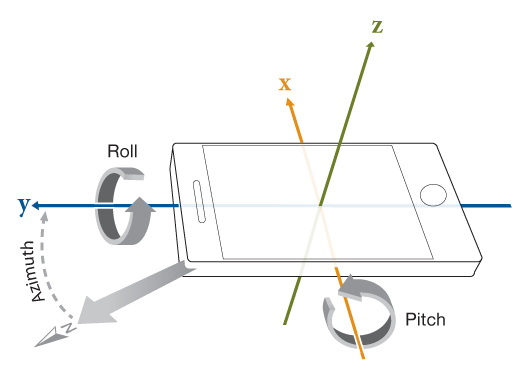
\includegraphics[width=8.5cm]{phoneOrientation}
	\caption{A device's body orientation.}\label{fig:fig1}
\end{figure}


\section{Approach}

To build a model to determine whether two devices share the same context, we
took the following approach:

\begin{enumerate}
\item Modify the MPU9250 library to work with the PowerDue.
\item Establish a clock on the PowerDue, to allow us to synchronize readings
      from the MPU9250 with readings from PowerSense.
\item Run three experiments to collect data from the MPU9250 and PowerSense iOS
      app. See Figure~\ref{fig:fig2} and Figure~\ref{fig:fig3} for an example of
      the type of data collected with PowerSense.
\item Use the unix timestamps to aggregate MPU9250 and PowerSense data.
\item Normalize the data.
\item Build a neural network architecture.
\item Train the neural network.
\item Evaluate the model.
\end{enumerate}

\subsection{Modifying MPU9250 library}

The MPU9250 library, which implements an interface to interact with the MPU9250
sensor, which contains a 3D gyroscope, accelerometer, and magnetometer, required
only one modification to work with the PowerDue, updating the instances of the
\texttt{Wire} interface with \texttt{Wire1}, given that PowerDue has two wire
interfaces. In addition to this modification, we used a library example module
\cite{MPU9250Ex} as the basis for the PowerDue module that we used to obtain
readings from the MPU9250 sensor. We disabled most of the logic in the example
module, but nonetheless relied on critical sections of the module, such as
initializing and calibrating the sensor.

\subsection{Time Synchronization}

In order to be able to compare the readings from both devices, each reading had
to be timestamped, and the timestamps from the devices had to be relatable,
i.e., one timestamp could be converted to the other. PowerSense readings
provided a unix timestamp by default, and this was ideal, but the PowerDue did
not not have a system clock established, i.e., calling a clock time function
would begin counting time from zero.

To establish the system clock on the PowerDue, we used RTCDue, a library that
allows you to set the time in different ways \cite{RTCDue}, e.g., using a
unixtime stamp or a date. Ideally, we would have prefered to use the NTP
protocol to set the time on the PowerDue, because the time would have a greater
degree of accuracy. Unfortunately, we were unable to use NTP because we were
unable to get the Wi-Fi module to work. We tried approaches in different example
modules found within the PowerDue libraries, but none of them worked. Therefore,
we resorted to a compile-time mechanism for setting the time.

To set the time at compile-time, we passed in the macros \texttt{\_\_TIME\_\_}
and \texttt{\_\_DATE\_\_} to couple of RTCDue library functions to set the time
and date. Essentially, we would used the compiler to pass in the time when it
built the binary. Simply setting the time like this did not yield a very
accurate time, because of the delay between macro substitution at compile-time
and program execution. To offset this delay, we reset the time at runtime by
adding seconds to the time set with \texttt{\_\_TIME\_\_} and
\texttt{\_\_DATE\_\_}, essentially using inspection to pick the number of
seconds that made the time reported by PowerDue closer to the time reported by
our machines and PowerSense.

After setting the system clock, it was simply a matter of using the Time library
function \texttt{now} \cite{TimeLib} to output the unix timestamp with the
readings from the MPU9250. Ideally, we would have preferred a millisecond
accuracy level, which we might have obtained using NTP, but the compile-time
method of setting the time provided accuracy of within a second, allowing us to
carry on with the experiments.

\begin{figure}[!t]\centering
	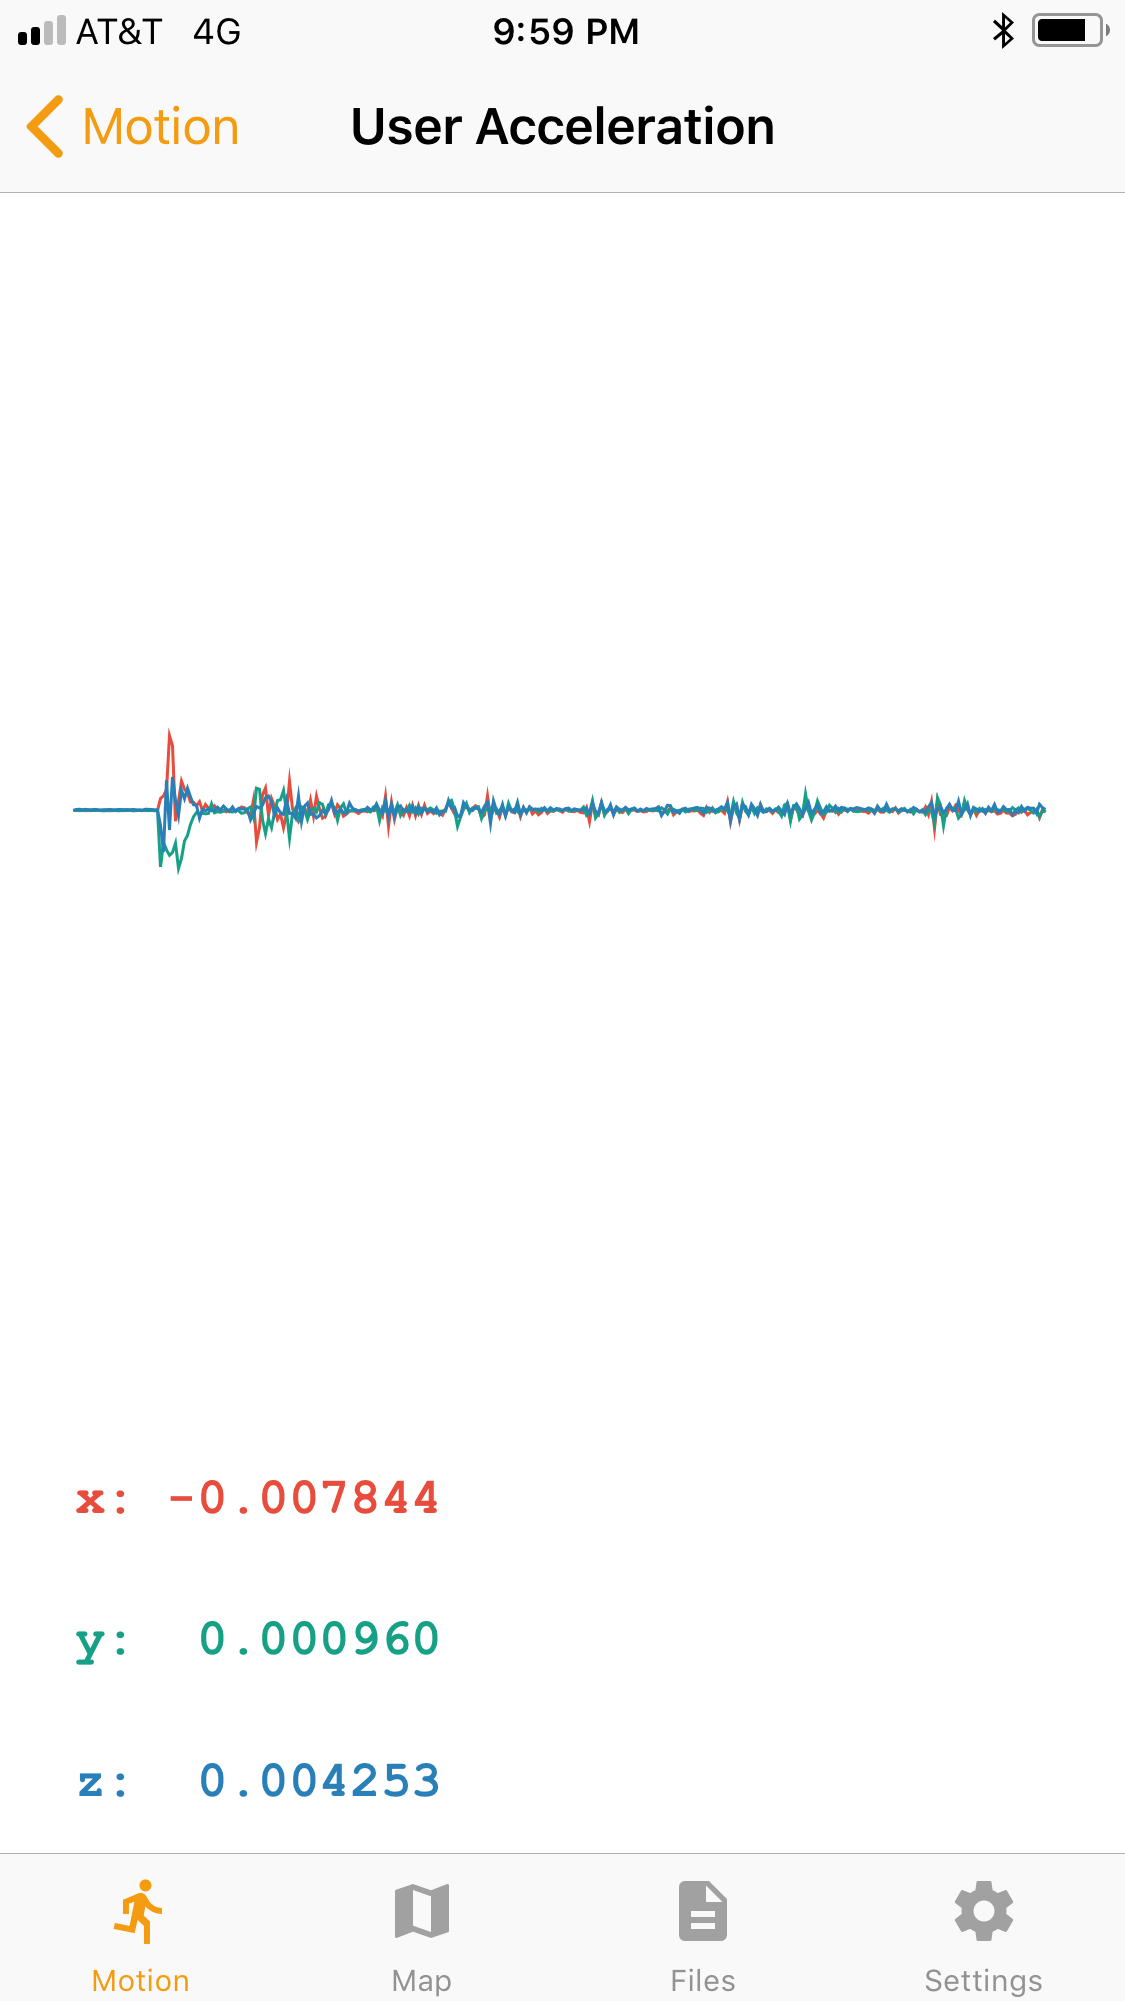
\includegraphics[width=5.5cm]{acceleration}
	\caption{User acceleration with iOS app PowerSense.}\label{fig:fig2}
\end{figure}

\subsection{Experiments}

We conducted three sets of experiments from which we collected data. We defined
shared context to mean that both devices, the PowerDue and the mobile phone,
were inside of the same car. The experiments were:

\begin{itemize}
\item \textit{Shared context}. Drive vehicle with both devices inside of
      vechicle.
\item \textit{No shared context}. Drive vehicle with PowerDue inside vehicle,
      while mobile phone is carried by pedestrian.
\item \textit{No shared context}. Drive vehicle with PowerDue inside vehicle,
      and drive another vehicle with mobile phone inside it.
\end{itemize}

An essential ingredient of all the experiments was movement, in order to provide
stimulus for the sensors, and hence our decision to carry the experiments while
driving or walking. We repeated each experiment five times, and for each
experiment trial collected about a minute's worth of readings from each device.

The output of each experiment was a set of data files. PowerSense allowed us to
email the readings of an experiment as a CSV file to ourselves. For PowerDue, we
had to manually create a CSV file by copying the output from the serial console
to the file.

\subsection{Aggregating data}

There are a number of reasons why we aggregated the data from two data files to
one data file per experiment. One is convenience (e.g., uploading one data file
as a data frame vs multiple data files), but more importantly, to match the
readings from each device, which we did in a three step process.

\begin{enumerate}
\item Find the timestamps (i.e., seconds) where both devices output readings.
\item From each device's data file, select the readings with a timestamp from
      step 1.
\item In cases where the number of readings for a given second don't match,
      apply a transformation to make the number of readings for that second
      equal for both devices.
\end{enumerate}

Even though we tried to start and stop reading from each device at the same
time, it is inevitable to have slight variation when taking samples from more
devices, especially if there is a human element to the experiment, which there
was in our expriments because we started the readings manually by flashing the
program on the PowerDue and pressing a button the on the PowerSense app.
Therefore, we used only readings with timestamps in existing in both data files,
per step 2.

In step 3, we had to apply some transformations because PowerSense produced 50
readings per second, while PowerDue only produced 38 readings per second. To
smooth-out this difference, we mapped pairs of readings from PowerSense into a
single reading with the average of both readings, but we applied this only to
the tail end of the readings from PowerSense. For example, suppose $PD_s$ is the
set of readings $a_1, a_2, ..., a_{38}$ from the PowerDue, and $PS_s$ is the set
of readings $b_1, b_2, ..., b_{50}$ from PowerSense, for second $s$, and $a_i$
and $b_i$ represent vectors. Then the transformation applied to $PS_s$ would map
the last 24 readings to 12 readings, as indicated below:

\begin{align}
    b'_{26} &= \frac{b_{26} + b_{27}}{2} \\
    b'_{27} &= \frac{b_{28} + b_{29}}{2} \\
    \vdots \\
    b'_{38} &= \frac{b_{49} + b_{50}}{2}
\end{align}

\subsection{Data normalization}

After aggregating data by time, we normalized the data in two ways:

\begin{itemize}
\item Normalized all the data values (i.e., x, y, z and values for orientation,
      acceleration, and magnetic), so that the mean would be zero and the
      standard deviation 1.
\item Made all input arrays, obtained from each aggregate experiment file, have
      the same dimensions.
\end{itemize}

We normalized all the data values because having training data with a mean of
zero tends to seep up convergence \cite{DLTricks}. We also normalized every
input array to have the same number of rows, in order to be able to use a neural
network architecture with an convolutional layer and a dense output layer. To
make all the arrays have the same number of rows, we computed the average number
of rows per array (15 total arrays, one per experiment trial), and removed rows
from the end of arrays with more rows, or repeated the last row at the end of
arrays with less rows.

\subsection{Neural network architecture}

Our neural network architecture consists of 5 layers:

\begin{enumerate}
\item Input convolutional layer with a relu activation function.
\item Hidden convolutional layer with a relu activation function.
\item Hidden max pooling layer.
\item Hidden dense layer with a relu activation function.
\item Output dense layer with softmax activation function.
\end{enumerate}

With Keras \cite{Keras}, it was trivial to implement the network, as the
following lines of python code demonstrate

\begin{lstlisting}
model = Sequential()
model.add(Conv2D(32, kernel_size=(3, 3),
             activation='relu',
             input_shape=input_shape))
model.add(Conv2D(64, (3, 3), activation='relu'))
model.add(MaxPooling2D(pool_size=(2, 2)))
model.add(Dropout(0.25))
model.add(Flatten())
model.add(Dense(128, activation='relu'))
model.add(Dropout(0.5))
model.add(Dense(2, activation='softmax'))
\end{lstlisting}

Even though the data we collected is inherently time dependent, the way our
experiments were carried makes time less of an important variable, because we
did not carry out any experiments in which we tested changing context, i.e.,
going from sharing context to not sharing context. Such an experiment would have
required us to look at how the variables change over time, precisely so that we
could devise a model that can distinguish the moment when a device's state
changes from being in context to not being in context.

In our experiments, the devices are either in context, or not in context, there
is no change from one to the other. This motivated our decision to use a
convolutional neural network, where time is not a factor. We simply wanted to
classify the input as either in context, or not in context, hence an output
layer using a softmax function \cite{DeepLearning,LeCunn}.

From the code, it may seem like the network also has a \texttt{Dropout} layer;
however, dropout is not inherently part of the network, but rather a technique
used to randomly drop units of the network during training in order to prevent
overfitting of the model \cite{Droptout}.

\subsection{Training the network}

\subsection{Evaluating results}


\section{Pending work}

Up until this point, our work has consisted of research, and more of it
remains to be done; however, there are key steps that we need to follow through
with in order to deliver results on the research:

\begin{enumerate}
\item Obtain a sensor with a gyroscope and accelerometer. None of the sensor at
      our disposal contain a gyroscope, which is the center piece of
      orientation-sensing algorithms. Therefore, it is imperative that we obtain
      one soon, because using a new sensor might entail having to modify or
      create drivers for the PowerDue.
\item Compute the attitude of the PowerDue.
\item Compute the attidue of a mobile phone.
\item Correlate the readings from the PowerDue and mobile phone.
\end{enumerate}

Our plan is to run experiments in which we repeat steps 2 - 4 under different
conditions, but in all the PowerDue and the mobile phone are stationary when the
sensor data is collected:

\begin{itemize}
\item Both devices have the same orientation and are in the same context.
\item Both devices are in the same context, but their orientations differ.
\item Devices are not in the same context, but have the same orientation.
\item Devices are not in the same context, and have different orientations.
\end{itemize}

To deliver useful results, we have to correlate the data between different
devices, and define what it means for two devices to share context. Also note
that we plan to correlate the data between the devices by doing the
analysis on our PCs, but ideally it would be more useful to deploy the model
on the PowerDue, perhaps a task for future work.

\section{Conclusion}

\begin{figure}[!t]\centering
	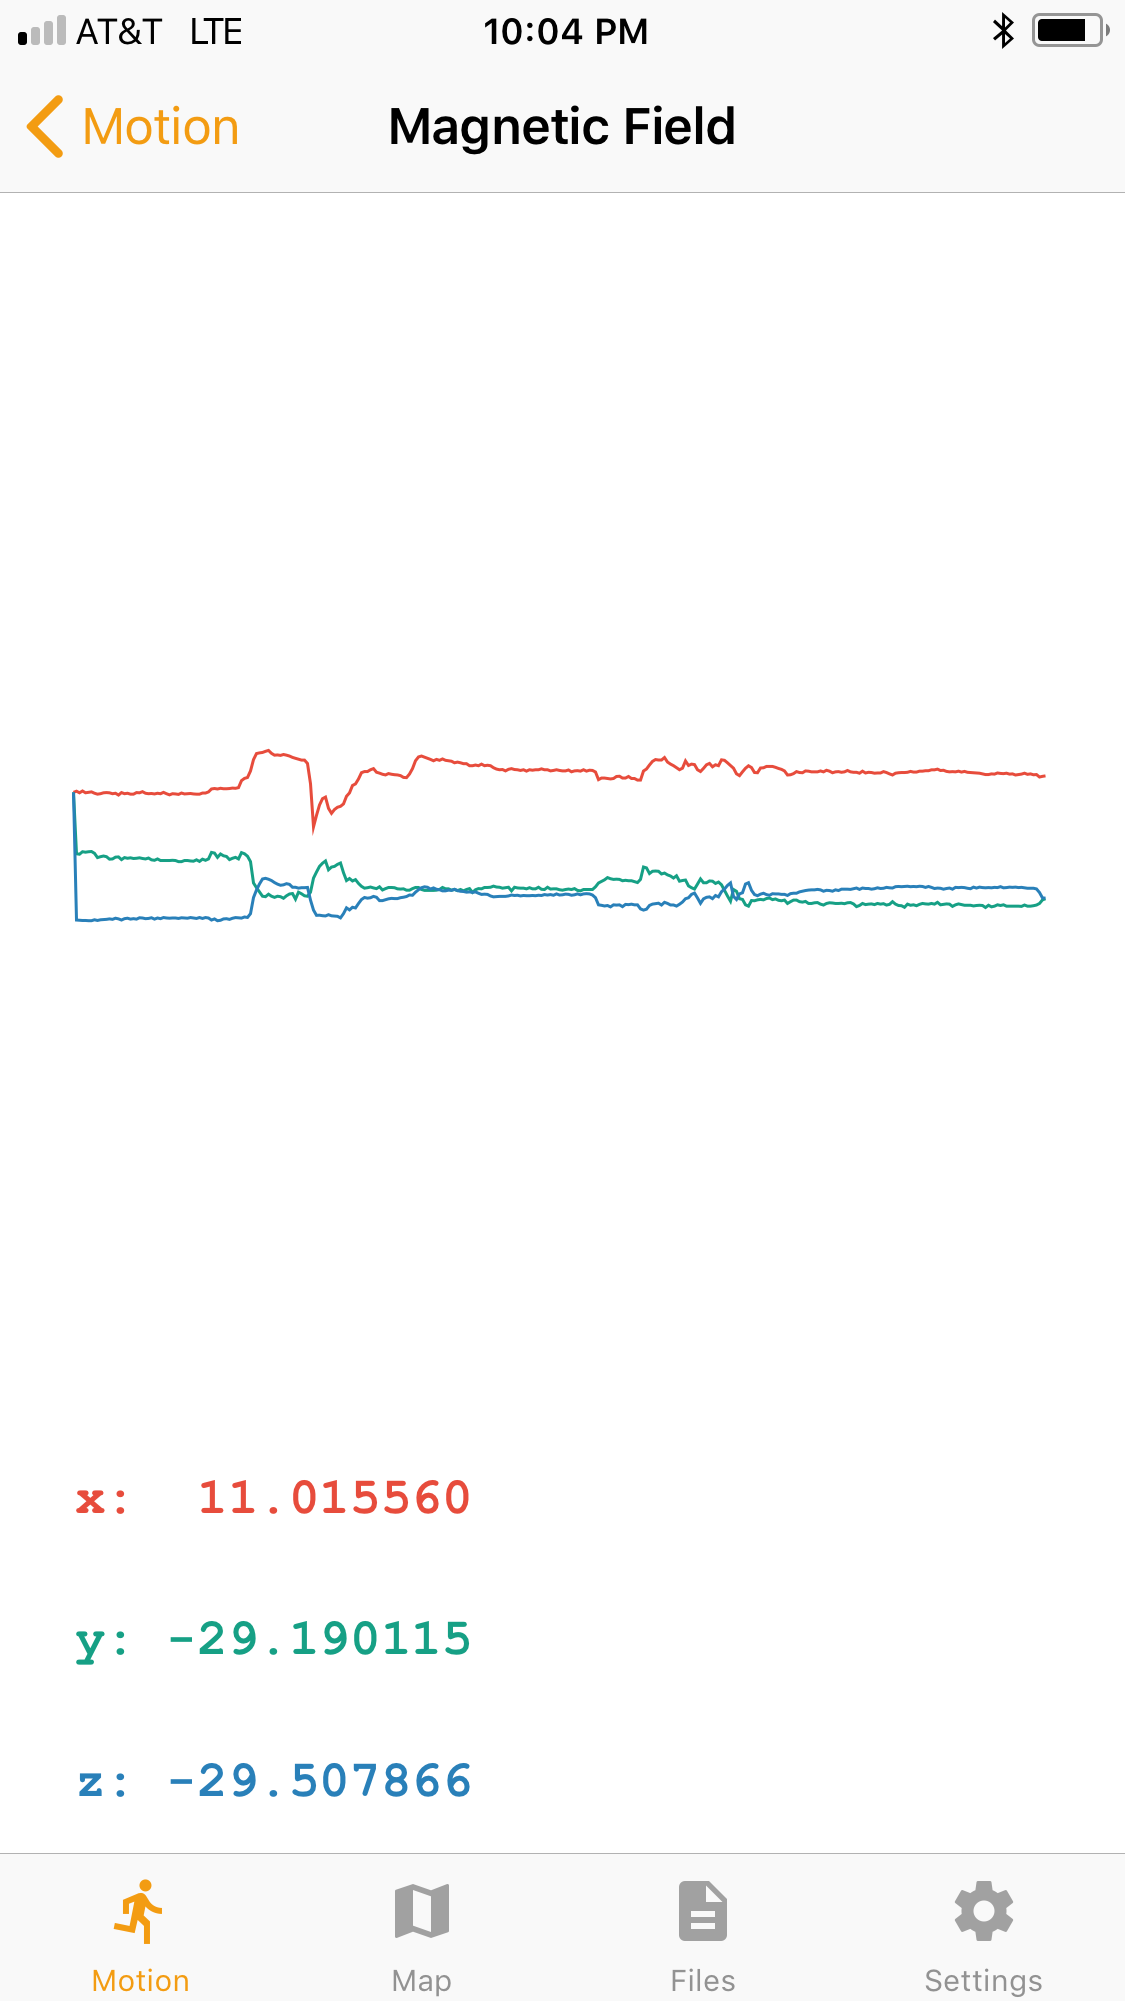
\includegraphics[width=5.5cm]{magnetic_field}
	\caption{Magnetic field with iOS app PowerSense.}\label{fig:fig3}
\end{figure}

% References

\bibliographystyle{Bibliography/IEEEtranTIE}
\bibliography{Bibliography/IEEEabrv,Bibliography/BIB_1x-TIE-2xxx}\ %IEEEabrv instead of IEEEfull

\end{document}
